\documentclass[runningheads]{llncs}

\usepackage[T1]{fontenc}
\usepackage{amsmath}
\usepackage{graphicx}
\usepackage{booktabs}
\usepackage{array}
\usepackage{url}
\def\UrlBreaks{\do\/\do-\do_}

\begin{document}

\title{The Exploitability Gap in LLM-Serving Scheduler Portfolios}
\titlerunning{The Exploitability Gap in LLM-Serving Scheduler Portfolios}

\author{Soroush Vahidi\inst{1}}
\authorrunning{S. Vahidi}
\institute{New Jersey Institute of Technology, Newark, NJ, USA\\
\email{sv96@njit.edu}}

\newcommand{\anwg}{ANWG}
\newcommand{\sbs}{SBS}
\newcommand{\vbs}{VBS}
\newcommand{\policy}[1]{\texttt{\detokenize{#1}}}

\maketitle

\begin{abstract}
LLM-serving schedulers have complementary strengths, motivating portfolios. On
a 240-scenario joint workload, per-scenario best-policy choice improves
arrival-normalized weighted goodput (ANWG) by 0.0190 over the best fixed
policy (SBS). Lightweight online adapters fall below SBS, and a stronger
nonlinear cost-sensitive utility selector reaches near-SBS ANWG but recovers
only $\approx$2.5\% of SBS$\rightarrow$VBS headroom (gain CI includes zero).
On the same joint-240 scenarios, terminal one-step counterfactuals are sparse
and concentrated; native disagreement predicts them only moderately.
Real-vLLM validation separately shows simulator--engine semantic mismatch and
a native token-budget tradeoff.

\keywords{LLM serving \and scheduling \and portfolios \and vLLM}
\end{abstract}

\section{Introduction}
\label{sec:introduction}

LLM inference serving has to schedule heterogeneous work. Requests differ in
prompt length, predicted and realized generation length, SLO or deadline
tightness, class or tenant weight, KV-cache footprint, burst timing, and
interactions between prefill and decode. These dimensions stress different
mechanisms in the serving stack: one workload may reward uninterrupted prompt
processing, another may reward urgent-deadline protection, and another may
reward preserving scarce KV capacity. It is therefore unlikely that one simple
scheduling rule will dominate all operating regimes.

This makes scheduler portfolios appealing, echoing algorithm-selection work
that compares a single best solver against a virtual best solver
(\sbs{} versus \vbs{})~\cite{rice1976algorithmselection,gomes2001portfolios,satzilla2008,autofolio2015}.
The \vbs{} measures \emph{scenario-level policy complementarity} as offline
opportunity; an online adaptive scheduler must act from online-observable
information under closed-loop queue dynamics. Whether that opportunity is
recoverable is a distinct \emph{exploitability} question, formalized in
Section~\ref{sec:metrics}.

Even when regimes are detectable, a router may fail to recover utility because
high-value intervals are sparse, closed-loop execution shifts decision support,
or coarse labels misalign with online decision boundaries. We therefore ask
whether tested adaptive mechanisms can exploit portfolio structure under
online-observable serving information.

We study a fixed six-policy portfolio motivated by LLM-serving mechanisms such
as iteration-level scheduling, PagedAttention, and chunked
prefill~\cite{orca2022,vllm2023,sarathi2024}, together with disaggregated and
fairness-oriented serving ideas~\cite{distserve2024,vtc2024}.
The portfolio spans full and chunked prefill, estimated-service ordering,
weighted fair sharing, least-laxity urgency, and KV-aware admission. We
evaluate complementarity across controlled and joint workloads and local
vLLM, then test adaptive exploitation, terminal-criticality analysis, and
constructive alternatives under preregistered splits, detailed in the four
contributions below. Except where noted, results are interpreted across
separately scoped settings (Section~\ref{sec:metrics}); they do not constitute
one shared numeric decomposition of joint-workload headroom.

This paper makes four contributions:
\begin{enumerate}
  \item We show workload-dependent complementarity and positive \vbs{} headroom
  for a six-policy portfolio, under jointly varying pressures and after
  expanding the envelope with independently motivated external baselines.
  \item On the same joint workload used to measure that headroom, we compare
  \sbs{}, \vbs{}, lightweight selectors/routers, and a stronger nonlinear
  cost-sensitive utility selector ($A_{\mathrm{hgb}}$): the stronger learner
  improves over the lightweight methods and reaches near-\sbs{} mean ANWG,
  but its gain over \sbs{} is indistinguishable from zero and closes only a
  small fraction of measured \vbs{} headroom.
  \item On the same joint-240 scenarios, a terminal counterfactual
  fork-and-continue analysis finds sparse, concentrated one-step effects and
  only moderate disagreement-proxy quality; a controlled A/B/C study
  corroborates the pattern. Terminal effects remain continuation-policy
  conditional.
  \item We test constructive exploitation beyond selection (support expansion,
  guarded composition, typed synthesis) and validate a simulator-derived
  mechanism against native vLLM; results remain bounded negative, or reveal a
  semantic mismatch and a native token-budget tradeoff.
\end{enumerate}

\section{Portfolio, Workloads, and Metrics}
\label{sec:methods}

\subsection{Problem setting}

We model LLM-serving as an online scheduling problem over arriving requests,
each with an arrival time, prompt-token length, predicted generation length,
class/tenant identifier, priority weight, and SLO deadline. During execution
the simulator exposes online-observable state---queued and admitted/running
requests, elapsed waiting time, remaining or predicted service proxies, active
sequence counts, prefill/decode phase, and KV capacity/pressure---and a policy
chooses which request to admit or serve next, how prompt work is chunked when
that control exists, and whether KV/load constraints allow admission.

The policy input is intentionally online-observable. The future actual output
length of an unfinished request is not exposed; it is used only after a run to
compute outcomes. Thus offline \vbs{} quantities, including the best policy for
a scenario, are analytical baselines rather than scheduler inputs.

\subsection{Six-policy portfolio}

The fixed portfolio contains six policies spanning distinct mechanisms.
Table~\ref{tab:policy-matrix} summarizes the paper-facing interpretation;
implementation details remain in the repository artifacts.

\begin{table}
\centering
\scriptsize
\caption{Six-policy portfolio used for envelope and complementarity analysis.
Online state is restricted to quantities observable during serving; future
actual output length is never an input.}
\label{tab:policy-matrix}
\setlength{\tabcolsep}{4pt}
\renewcommand{\arraystretch}{0.9}
\begin{tabular}{@{}p{0.20\textwidth}p{0.42\textwidth}p{0.28\textwidth}@{}}
\toprule
Policy & Mechanism & Key online state \\
\midrule
Full prefill & Uninterrupted prompt processing for long prompt-heavy work & Queue order, prompt phase, prefill budget \\
Small-chunk prefill & Prompt chunking for prefill/decode interleaving and late TTFT & Queue order, prompt phase, chunk budget \\
ESTF & Short estimated-service first for completion efficiency & Prompt tokens, predicted output tokens \\
WFS & Weighted service-deficit fairness and SLO protection & Class weights, admitted/completed service \\
LLF & Least-laxity urgency under deadlines & Deadline, current time, predicted service \\
KV constrained & KV-reserve admission/scheduling with urgent bypass & KV capacity, estimated KV demand, laxity \\
\bottomrule
\end{tabular}
\renewcommand{\arraystretch}{1}
\end{table}

These are repository-specific baselines, not full reproductions.
\policy{full_prefill} follows iteration-level batching in Orca/vLLM~\cite{orca2022,vllm2023}.
\policy{chunked_prefill_small} is motivated by
chunked-prefill work such as Sarathi-Serve~\cite{sarathi2024} (our simulator
omits its full stall-free decode-priority algorithm). ESTF follows SPT/SRPT
intuition~\cite{schrage1968queuejumping}; WFS follows GPS/WFQ-style
fairness~\cite{parekh1993gps,demers1989fairqueueing,vtc2024}; LLF is a
real-time urgency heuristic; KV constrained relates to KV-aware
serving~\cite{vllm2023,kvscheduling2025}.

\subsection{Workload suites}

We use four workload categories. First, public trace replay provides a realism
baseline using BurstGPT and Azure 2023 LLM-inference traces
~\cite{burstgpt2025,azurepublicdataset2023,splitwise2024}. We construct 20
200-request windows from each of BurstGPT, Azure conversation, and Azure code,
retaining source order, relative timestamps, and prompt/output token counts;
predicted lengths, deadlines, priorities, and classes are deterministic
overlays, and actual future output length is hidden from online policies.
This configuration motivates stress workloads but does not show public traces
are generally uninformative.

Second, controlled Families A/B/C isolate mechanisms. Family A stresses
fairness, completion, and SLO conflict; Family B stresses prefill/decode
contention; and Family C stresses KV pressure and urgency. These families are
the original controlled evidence for complementarity and later
selector/router/synthesis tests.

Third, the joint multi-mechanism workload broadens the evidence beyond
concatenated stress families. It contains 240 scenarios drawn from one common
schema that jointly varies offered load, burstiness, long-vs-short mixture,
prompt-length heterogeneity, output/service-length heterogeneity, tenant weight
skew, SLO tightness, prediction noise, KV pressure, late-arrival structure,
active-sequence capacity, and step-token budget. Its pressure audit is
outcome-independent: it computes six normalized indicators in $[0,1]$
covering fairness, service heterogeneity, prefill/decode contention, KV
pressure, urgency, and burst pressure. A pressure is counted as elevated when
the corresponding indicator is at least 0.60, as specified before policy
evaluation. Under this audit, 223 of 240 scenarios (92.9\%) have at least two
elevated mechanism pressures, and 175 have at least three.

Fourth, local real-vLLM validation on Qwen2.5-0.5B served by vLLM 0.27.1 on an
RTX 5060 Ti tests whether the simulator's prefill/decode abstraction
corresponds to native behavior and whether native vLLM exposes its own
scheduling-control tradeoff; these experiments are not used to tune the
simulator.

Across these studies, practical-effect and robustness criteria were specified
before held-out or screening evaluations; selector/router analyses distinguish
offline labels from live closed-loop re-evaluation. Joint-workload CIs use
1{,}000 scenario-bootstrap resamples; native-vLLM CIs use percentile bootstraps
over five paired repetition-level differences after matched warmups and ABBA
ordering.

\subsection{Metric and envelope definitions}
\label{sec:metrics}

The primary utility is arrival-normalized weighted goodput (\anwg{}):
\begin{equation}
\label{eq:anwg}
  \mathrm{\anwg{}} =
  \frac{\sum_i w_i \mathbf{1}[i\ \mathrm{completed}] \mathbf{1}[C_i \le D_i]}
       {\sum_i w_i}.
\end{equation}
Dropped, unfinished, or late completions receive zero numerator credit but
remain in the arrival-weight denominator.

For evaluation set $X$, portfolio $P$ (here $P_6$), policy utility $R_h(x)$,
and adaptive utility $R_A(x)$, the single best scheduler (\sbs{}) and virtual
best scheduler (\vbs{}) are
\begin{equation}
\label{eq:sbs}
  h^* = \arg\max_{h \in P} \frac{1}{|X|}\sum_{x \in X} R_h(x),
  \quad
  R_{\mathrm{\sbs{}}}(X,P)
  =
  \frac{1}{|X|}\sum_{x \in X} R_{h^*}(x),
\end{equation}
\begin{equation}
\label{eq:vbs}
  E_P(x) = \max_{h \in P} R_h(x),
  \quad
  R_{\mathrm{\vbs{}}}(X,P)
  =
  \frac{1}{|X|}\sum_{x \in X} E_P(x).
\end{equation}
We write $E_6(x)$ when $P=P_6$. An $\epsilon$-unique winner satisfies
$R_h(x) \ge \max_{q\ne h} R_q(x)+\epsilon$ ($\epsilon=0.01$ \anwg{}).
\vbs{} headroom is
\begin{equation}
\label{eq:headroom}
  \mathrm{Headroom}(X,P)
  =
  R_{\mathrm{\vbs{}}}(X,P) - R_{\mathrm{\sbs{}}}(X,P).
\end{equation}
\emph{\vbs{} headroom measures portfolio opportunity; the exploitability gap is
defined relative to a particular adaptive mechanism on the same $X$.}
Realized gain is $R_A(X)-R_{\mathrm{\sbs{}}}(X,P)$; selector regret is mean
$E_P(x)-R_{\hat h(x)}(x)$ for selected parent $\hat h(x)\in P$.
The exploitability gap is
\begin{equation}
\label{eq:eg}
  \mathrm{EG}(A;X,P)
  =
  R_{\mathrm{\vbs{}}}(X,P) - R_A(X)
  =
  \frac{1}{|X|}\sum_{x \in X}(E_P(x)-R_A(x)).
\end{equation}
Each headroom or gap metric is scoped to its own $X$; equating values across
datasets is invalid unless evaluations share $X$ and $P$.
When $\mathrm{Headroom}(X,P)>0$, normalized \vbs{}-gap closure is
\begin{equation}
\label{eq:gapclosure}
  \mathrm{GapClosure}(A;X,P)
  =
  \frac{R_A(X) - R_{\mathrm{\sbs{}}}(X,P)}
       {R_{\mathrm{\vbs{}}}(X,P) - R_{\mathrm{\sbs{}}}(X,P)},
\end{equation}
with residual $\mathrm{NEG}(A;X,P)=1-\mathrm{GapClosure}(A;X,P)$.
Zero headroom makes closure undefined; values below $0$ or above $1$ indicate
underperformance or out-of-envelope behavior and require cautious
interpretation. Synthesized marginal envelope gain averages
$\max(R_c(x),E_P(x))-E_P(x)$ over the pre-specified training screen.

\section{Portfolio Complementarity}
\label{sec:complementarity}

An adaptive portfolio requires useful parent disagreement. We ask whether
policies produce workload-dependent winners under controlled mechanisms and
whether that complementarity persists under jointly varying pressures.

\subsection{Controlled mechanism families}

The controlled A/B/C suites isolate specific serving tensions. Family A varies
fairness, completion, and SLO conflict; Family B varies prompt-heavy prefill
pressure against late short requests; and Family C varies KV pressure and
urgent arrivals. Across the unified 176-scenario, six-policy matrix, the
portfolio produces 1,056 policy cells and a 54.0\% $\epsilon$-unique-winner
rate. The best fixed policy and \vbs{} headroom differ by family: WFS is best
fixed in Family A with 0.021742 headroom, full prefill is best fixed in Family
B with 0.049433 headroom, and \policy{kv_constrained_online} is best fixed in
Family C with 0.020261 headroom; these results isolate mechanisms, not a
production-traffic claim.

\subsection{Public-trace saturation}

Public-trace replay is a sanity check, not the main discriminating benchmark.
Under the processed replay configuration, all 60 windows tie at \anwg{} 1.0,
six-policy envelope gain is 0.0, active count p99 is 5 out of 512, and maximum
KV utilization is 0.003802: this configuration does not expose scheduler
differentiation for the current objective.

\subsection{Joint multi-mechanism workload}

To test whether complementarity is merely an artifact of disjoint handcrafted
families, we generated a 240-scenario joint workload from one common schema
before evaluating policy outcomes (Figure~\ref{fig:joint-complementarity}).
Per-scenario winners remain distributed across the portfolio: LLF wins 59
scenarios, \policy{kv_constrained_online} 50, full prefill 46, ESTF 45, WFS
35, and small-chunk prefill 5. The $\epsilon$-unique-winner fraction is
59.6\%, nontrivial policy spread appears in 91.7\% of scenarios, and the mean
policy range is 0.111658 \anwg{}.

\begin{figure}[t]
\centering
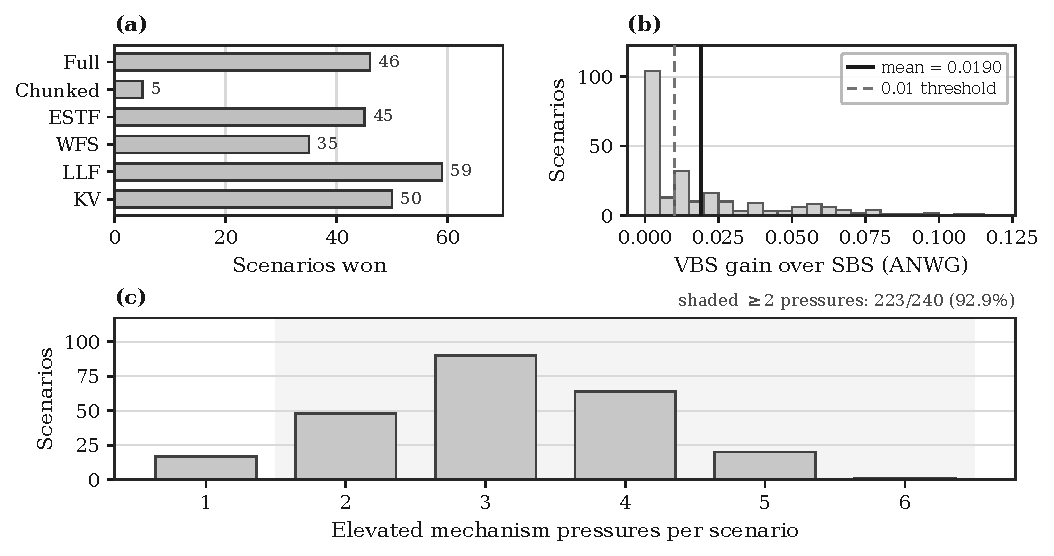
\includegraphics[width=\textwidth]{figures/joint_complementarity.pdf}
\caption{Joint 240-scenario multi-mechanism workload under $P_6$ (excludes the
external expansion, Section~\ref{sec:external-portfolio}).
(a)~Per-scenario \vbs{} winner counts.
(b)~Per-scenario \vbs{} gain over \sbs{} (ANWG); solid = mean, dashed = $0.01$.
(c)~Elevated mechanism pressures per scenario (threshold $0.60$); shading
marks $\geq 2$ pressures.
Winner diversity and positive headroom persist under jointly varying
pressures.}
\label{fig:joint-complementarity}
\end{figure}

The \sbs{} over the joint workload is
\policy{kv_constrained_online}, with mean \anwg{} 0.314072. The six-policy
\vbs{} reaches mean \anwg{} 0.333106, yielding \vbs{} headroom 0.019034 with
bootstrap 95\% CI [0.015988, 0.022433]. The median per-scenario \vbs{} gain is
0.010622, p90 gain is 0.058040, 60.4\% of scenarios have positive gain, and
51.3\% have gain at least 0.01. Most gain arises outside single-mechanism
extremes: 93.1\% comes from scenarios with at least two elevated pressures and
63.3\% from scenarios with at least three; the top 10\% of scenarios account
for 40.5\% of total gain: bounded synthetic evidence, not a production claim.

\subsection{External-portfolio robustness}
\label{sec:external-portfolio}

A natural concern is that $P_6$ opportunity is an artifact of weak baselines.
We expand the portfolio on the same joint-240 scenarios to
$P_{\mathrm{ext}}=P_6\cup\{\mathrm{VTC},\textrm{vLLM-style}\}$, using an
official VTC implementation~\cite{vtc2024} and a disclosed continuous-batching
proxy. Learning-to-rank and SOLA-style systems
remain separate evidence~\cite{llmltr2024,sola2025}; they are not members of
$P_{\mathrm{ext}}$. Adaptive experiments in Sections~\ref{sec:gap}--\ref{sec:constructive}
remain scoped to $P_6$ and were not retroactively retrained over eight policies.

\begin{table}
\centering
\footnotesize
\caption{Joint-240 portfolio envelopes for $P_6$ and
$P_{\mathrm{ext}}=P_6+\mathrm{VTC}+\textrm{vLLM-style}$.
SBS policy is \policy{kv_constrained_online} in both cases.
Bootstrap 95\% CIs use 1{,}000 scenario resamples (seed 20260825).}
\label{tab:pext}
\setlength{\tabcolsep}{4pt}
\begin{tabular}{@{}lcccc@{}}
\toprule
Portfolio & SBS & VBS & Headroom & $\Delta$VBS vs.\ $P_6$ \\
\midrule
$P_6$ & 0.314072 & 0.333106 & 0.019034 & --- \\
$P_{\mathrm{ext}}$ & 0.314072 & 0.333319 & 0.019247 & $+0.000214$ \\
\bottomrule
\end{tabular}
\end{table}

Table~\ref{tab:pext} summarizes the envelope comparison. SBS is unchanged.
VBS rises only by $+0.000214$ (bootstrap CI $[0.00004,0.00046]$), essentially
the VTC incremental envelope alone; the vLLM-style proxy adds $\approx 0$.
Headroom remains $\approx 0.019$ (Pext CI $[0.0162,0.0226]$). Under
$P_{\mathrm{ext}}$, winners remain diverse (LLF 57, KV 48, ESTF 45, WFS 34,
full prefill 27, VTC 23, chunked 3, vLLM-style 3), and leave-one-out removal of
any $P_6$ policy still reduces VBS (largest drops: KV $\approx 0.0071$,
LLF $\approx 0.0058$). Thus strong external baselines do not collapse the
observed opportunity: they neither replace the SBS nor erase $P_6$ unique
envelope contribution. This is a portfolio-scope robustness test, not a claim
of superiority over production VTC or native vLLM.

\subsection{From opportunity to exploitability}

Section~\ref{sec:complementarity} establishes positive \vbs{} headroom,
including on joint-240. Section~\ref{sec:gap} first summarizes two earlier
adaptive tests on other scopes, then directly compares \sbs{}, \vbs{}, and two
online adaptive methods on the \emph{same} joint-240 held-out scenarios, and
finally uses a terminal counterfactual analysis to help explain why recovery
is difficult (Section~\ref{sec:metrics}).

\section{Adaptive Exploitation}
\label{sec:gap}

We next evaluate whether tested adaptive mechanisms can convert complementarity
into deployable utility under preregistered criteria and evaluation scopes
(Section~\ref{sec:metrics}).

\subsection{Earlier controlled adaptive tests}
\label{sec:earlier-adaptive}

On the unified 176-scenario controlled-family matrix, within-family holdouts
showed learnability (Families A/B at zero regret; Family C competitive), but
pooled cross-family selection failed: best pooled regret 0.0463 exceeded
best-fixed 0.0233 and majority 0.0127, and leave-one-family-out transfer was
unstable (Family-A held-out regret 0.4786 versus fixed 0.0767). A shared-feature audit found perfect family classifiability but no
utility-consistent cross-family neighbors, so this rescue did not yield a
robust cross-family selector.

Separately, a hierarchical router achieved macro-F1 0.9887 with no
catastrophic misrouting, yet on live closed-loop re-evaluation gained only
+0.00616 mean \anwg{} over the best global fixed policy (below the +0.01
criterion) and achieved \vbs{}-gap closure 0.143 (Eq.~\ref{eq:gapclosure}),
far below the 0.75 target---an instance of Eq.~\ref{eq:eg}: accurate regime
detection can coexist with large residual opportunity because labels are
coarser than online decision boundaries and closed-loop scheduling shifts the
state distribution under which specialized policies were valuable.

\begin{table}
\centering
\footnotesize
\caption{Cross-experiment summary of pre-specified adaptive-exploitation
criteria. Each row uses its own evaluation scope and is not comparable as a
shared-dataset leaderboard.}
\label{tab:adaptive-criteria}
\setlength{\tabcolsep}{4pt}
\renewcommand{\arraystretch}{1.0}
\begin{tabular}{@{}>{\raggedright\arraybackslash}p{0.17\textwidth}
  >{\raggedright\arraybackslash}p{0.155\textwidth}
  >{\raggedright\arraybackslash}p{0.275\textwidth}
  >{\raggedright\arraybackslash}p{0.285\textwidth}@{}}
\toprule
Method & Scope & Intermediate signal & Result \\
\midrule
Pooled selector &
A/B/C (176) &
Within-family learnability &
Regret 0.0463 vs.\ fixed 0.0233 / maj.\ 0.0127 \\
Hierarchical router &
Live &
Macro-F1 0.9887; 0 catastrophic &
+0.00616 \anwg{} ($<$\,0.01); GapClosure 0.143 \\
Terminal-\anwg{} fork &
TRAIN/VAL (144) &
27/734 (3.7\%) nonzero; disagr.\ AUROC 0.513 &
Top-1\% mass 48.3\%; H10-proxy Spearman 0.005 \\
Support expansion &
Family-A &
24{,}314 fingerprints; 156 domains &
1/104 closer; p90\,$=$\,0; 0/8 criteria \\
Guarded composition &
Family-A &
WFS regret reduction 3.11\% &
$<$\,10\% min.; quadrant order fail \\
Typed crossover &
24 TRAIN &
Exact parents; 4{,}320 evals &
Best marginal gain 0.0; no promotion \\
\bottomrule
\end{tabular}
\renewcommand{\arraystretch}{1}
\end{table}

Table~\ref{tab:adaptive-criteria} summarizes bounded negative evidence across
settings, including the same-distribution and terminal-criticality results
detailed next; it does not imply that all adaptive schedulers must fail.

\subsection{Same-distribution joint-240 test}
\label{sec:same-dist}

Section~\ref{sec:complementarity} measures \vbs{} headroom offline; here we
test whether it is recoverable by online adaptive methods evaluated on the
\emph{same} joint-240 scenarios, using preregistered 5-fold out-of-fold
cross-fitting (seed 20260825). We restrict to $P_6$ and evaluate: a
scenario-level logistic selector ($A_{\text{scen}}$; 17 pre-policy features;
frozen utility lookup), a live 6-way router ($A_{\text{live}}$; online
features; dwell $\geq20$ steps; closed-loop scoring; live-vs-matrix agreement
$4\times10^{-7}$), and a stronger nonlinear cost-sensitive \emph{direct-utility}
portfolio selector ($A_{\mathrm{hgb}}$; HistGradientBoosting regressor over the
same 17-feature allowlist plus a policy indicator, nested hyperparameter
selection within training folds, held-out choice $\arg\max_p \widehat{\anwg{}}(x,p)$).

\begin{table}
\centering
\scriptsize
\caption{Same-distribution joint-240 results ($n=240$ out-of-fold scenarios;
headroom $0.019034$; paired scenario bootstrap ($B=1{,}000$ for rows above
$A_{\mathrm{hgb}}$). SBS policy is \policy{kv_constrained_online}.
Gain/GapClosure are relative to \sbs{}; negative GapClosure means added regret.
$A_{\mathrm{hgb}}$ uses $B=10{,}000$.}
\label{tab:samedist}
\setlength{\tabcolsep}{3pt}
\renewcommand{\arraystretch}{0.9}
\begin{tabular}{@{}lcccc@{}}
\toprule
Method & \anwg{} & Gain [95\% CI] & GapClosure & Catastrophic \\
\midrule
\sbs{} & 0.3141 & --- & --- & --- \\
\vbs{} & 0.3331 & --- & --- & --- \\
Majority & 0.2909 & $-0.023$ [$-0.031,-0.016$] & $-1.22$ & 109/240 \\
$A_{\text{scen}}$ & 0.3059 & $-0.008$ [$-0.013,-0.003$] & $-0.43$ & 67/240 \\
$A_{\text{live}}$ & 0.2840 & $-0.030$ [$-0.038,-0.023$] & $-1.58$ & 118/240 \\
$A_{\mathrm{hgb}}$ & 0.3145 & $+0.0005$ [$-0.0023,+0.0033$] & $+0.025$ & 34/240 \\
\bottomrule
\end{tabular}
\renewcommand{\arraystretch}{1}
\end{table}

$A_{\text{scen}}$ and $A_{\text{live}}$ fall \emph{below} \sbs{} (CIs exclude
zero); catastrophic regressions ($R_A<R_{\mathrm{\sbs{}}}-0.01$) affect 28\%
and 49\% of scenarios. $A_{\mathrm{hgb}}$ substantially reduces that deficit
($A_{\mathrm{hgb}}-A_{\text{scen}}=+0.0086$ $[0.0038,0.0139]$;
$A_{\mathrm{hgb}}-A_{\text{live}}=+0.0306$ $[0.0232,0.0386]$) and matches
\sbs{} within sampling error, yet closes only $\approx$2.5\% of
\sbs{}$\rightarrow$\vbs{} headroom. A secondary ExtraTrees utility model is
similar but slightly weaker (ANWG $0.3127$). Thus stronger nonlinear
utility learning removes much of the logistic/live gap without recovering the
measured opportunity.

\subsection{Why the tested methods fail: terminal decision criticality}
\label{sec:terminal-crit}

To link Section~\ref{sec:same-dist}'s same-distribution gap to decision
structure, we evaluate one-step terminal counterfactuals on the
\emph{same} joint-240 scenarios. At acquired fork points we force an
alternative $P_6$ action, continue under a cloned live-router policy, and
measure
$C_t=\mathrm{\anwg{}}_{\mathrm{CF}}-\mathrm{\anwg{}}_{\mathrm{ref}}$
(reference replays matched on all 240 scenarios). The estimand is
continuation-policy conditional, not a policy-independent action value.

On 3{,}541 evaluated states, effects are sparse and concentrated within the
evaluated intervention sample: 206 nonzero (5.82\%;
scenario-clustered CI $[4.44\%,7.34\%]$), with the top 1\% of states carrying
42.1\% of absolute mass (CI $[34.0\%,50.4\%]$; $B=2{,}000$, seed 20260825).
Mean $|C_t|$ is 0.00141 $[0.00098,0.00194]$. Native disagreement predicts
nonzero effects only moderately
(AUROC $0.680$ $[0.677,0.684]$;
AUPRC $0.082$ $[0.064,0.131]$; no-skill prevalence $0.058$);
a joint-240 H10 short-horizon proxy is unavailable.
Replacing live-router continuation by SBS on the same 3{,}541 keys raises
nonzero prevalence to 17.4\% $[15.4\%,19.5\%]$ with weak ranking overlap
(Spearman of $|C_t|$ $0.221$; top-1\% Jaccard $0.108$): sparsity persists,
but critical-state identity is partly continuation-dependent.

A controlled TRAIN/VAL A/B/C study (734 states; 27 nonzero, 3.7\%;
top-1\% mass 48.3\% with wide CIs; disagreement AUROC $0.513$)
corroborates the pattern under a separate design; joint-240 remains the
primary same-workload evidence for Section~\ref{sec:same-dist}.

\section{Constructive Exploitation Beyond Selection}
\label{sec:constructive}

We next test stronger exploitation mechanisms beyond parent selection under
pre-specified criteria (Table~\ref{tab:adaptive-criteria}). Target-free
\textbf{support expansion} (24{,}314 fingerprints over 156 training domains)
moved only 1/104 held-out states closer (p90 improvement 0).
\textbf{Guarded semantic composition} on Family~A cut WFS regret by only
3.11\% (below the 10\% bar) and violated the required completion/SLO
quadrant order. A \textbf{typed program synthesis} screen with exact parent
reproduction (4{,}320 evals) yielded best mean marginal gains of 0.0113
(random), 0.0026 (mutation), and 0.0 (crossover); no candidate met promotion
criteria.

\section{Real-System Validation}
\label{sec:real}

On this local probe (Section~\ref{sec:methods}) we validated prefill/decode
contention, testing qualitative mechanism transfer, not exact magnitude
matching.

\subsection{Direct Family-B analogue}

Family B fixes a 512-token simulator step budget and varies prefill chunk size
(full 65{,}536 vs.\ small-chunk 64). The native analogue varied chunking and
the native token budget (4096 vs.\ 512). All 300/300 requests completed
with real queueing, but native chunking did not reproduce the simulator-like
late-TTFT reversal under pre-specified criteria.

\subsection{Semantic diagnosis}

Diagnosis revealed semantic mismatch: native vLLM V1 does not implement the
same fixed-budget FCFS abstraction, and the native scheduler token budget is
itself a control variable. Scheduler traces overlapped but were not equivalent
(FULL: 6 mixed prefill+decode steps, 0 partial chunks; CHUNKED: 16 mixed steps,
21 partial chunks). Prefill remained nontrivial (3{,}200-token prefill
$\approx$0.0767\,s vs.\ 0.00591\,s/token decode).

\subsection{Native token-budget control}

With chunked prefill enabled and all other controls fixed, varying only the
native token budget (512 vs.\ 4096) produced repeatable workload-dependent
latency effects (Figure~\ref{fig:vllm-semantics}): two regimes, 20 measured
regime-runs, 150/150 successful requests, ABBA ordering.

\begin{figure}[t]
\centering
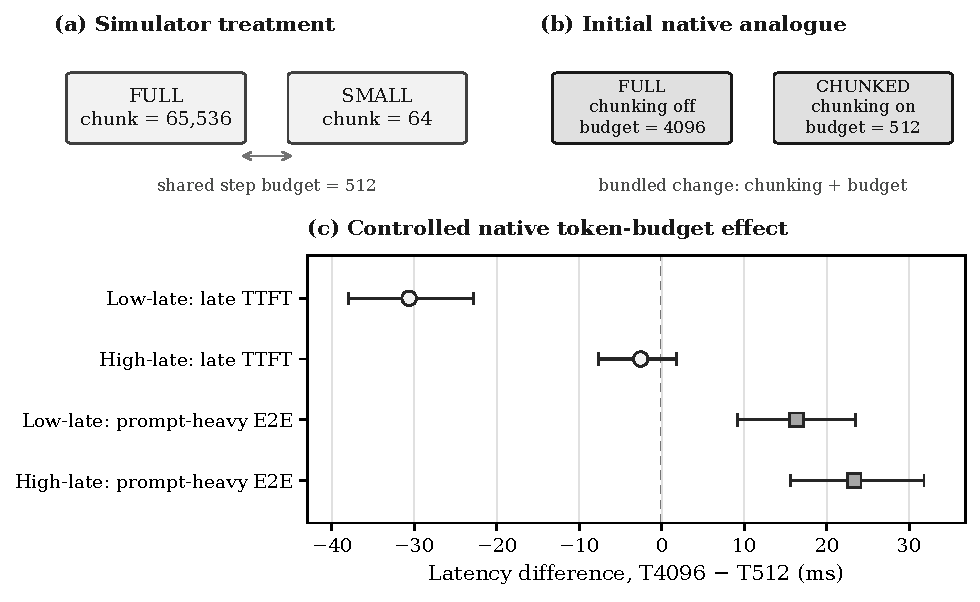
\includegraphics[width=\textwidth]{figures/vllm_semantic_validation.pdf}
\caption{Simulator-to-native vLLM validation on the local probe.
(a)~Simulator treatment: shared 512-token step budget, only prefill chunk
size varies.
(b)~Initial native analogue: chunking and token budget change together
(bundled, not single-factor).
(c)~Controlled native experiment, chunked prefill fixed; points are
T4096$-$T512 latency differences with 95\% bootstrap CIs.
Negative late-request TTFT favors T4096; positive prompt-heavy E2E favors T512.}
\label{fig:vllm-semantics}
\end{figure}

In the low-late regime, T4096 improved late-request TTFT by 30.6 ms (95\% CI
[-38.0, -22.8] ms; 5/5 sign consistency) but worsened prompt-heavy E2E by
16.3 ms (CI [9.2, 23.5] ms). In the high-late regime, late-TTFT change was
$-$2.5 ms (CI [-7.7, 1.8] ms; 3/5 consistency) while prompt-heavy E2E worsened
by 23.3 ms (CI [15.6, 31.8] ms). This is a native token-budget tradeoff in the
tested configuration, not a Family-B reproduction~\cite{vllm2023,sarathi2024,distserve2024,mooncake2025}.

\section{Related Work, Limitations, and Conclusion}
\label{sec:discussion}

\paragraph{Related work.}
Many LLM-serving systems already adapt online: migration
(Llumnix~\cite{llumnix2024}), queueing control (QLM~\cite{qlm2024}),
state-aware/multi-SLO scheduling (SOLA, SLOs-Serve~\cite{sola2025,slosserve2025}),
hierarchical multi-timescale routing (H-MAS~\cite{hmas2026}), flexible request
partitioning (Libra~\cite{libra2026}), and online policy self-evolution
(Autopoiesis~\cite{autopoiesis2026}). Others target one mechanism:
batching/memory (Orca, vLLM~\cite{orca2022,vllm2023}); chunked prefill and
prefill/decode isolation (Sarathi-Serve, DistServe, Splitwise,
TetriInfer~\cite{sarathi2024,distserve2024,splitwise2024,tetriinfer2024});
KV-centric serving (Mooncake~\cite{mooncake2025}); fairness via virtual
tokens (VTC~\cite{vtc2024}); preemption (FastServe~\cite{fastserve2026});
rank ordering~\cite{llmltr2024}; goodput/phase-aware scheduling (Past-Future,
PASCAL~\cite{pastfuture2025,pascal2026}); and KV-constrained
formulations~\cite{kvscheduling2025,wait2025}. To our knowledge, none jointly
quantifies \sbs{}/\vbs{} portfolio headroom, evaluates online adaptive
selectors against that opportunity on the same workload distribution, and
analyzes terminal counterfactual scheduling criticality---our focus. H-MAS is
closest for hierarchical adaptive routing but omits portfolio opportunity and
terminal criticality; Autopoiesis is closest for online policy synthesis,
more ambitious than our bounded screen (Section~\ref{sec:constructive}), but
likewise omits this formulation.

Methodologically, \sbs{}/\vbs{} envelopes follow classical algorithm selection
and portfolios~\cite{rice1976algorithmselection,gomes2001portfolios,satzilla2008}
as specialized in SATzilla, AutoFolio, and Hydra~\cite{autofolio2015,hydra2010};
we claim no novelty for those concepts, nor for decision-critical
states~\cite{karino2020criticalstates} or counterfactual action-value
estimation~\cite{mesnard2021counterfactual} in sequential decision-making
generally, neither of which targets LLM-serving scheduling. Serving differs:
actions change future queue and
resource state, so regime accuracy need not imply action accuracy---a
closed-loop covariate-shift motif familiar from imitation
learning~\cite{ross2011dagger}. Our contribution is a
terminal counterfactual-\anwg{} characterization of such
consequential decisions specifically within LLM-serving scheduler portfolios,
showing that native disagreement and a short-horizon completion proxy are
unreliable surrogates for it here. Typed synthesis inherits GP and
hyper-heuristic precedents~\cite{koza1992gp,montana1995stgp,whigham1995grammar,branke2015hyperheuristic};
our screen differs mainly by exact parent reproduction, a portfolio-envelope
objective, and pre-specified nonredundancy criteria rather than by inventing
evolutionary search~\cite{funsearch2024,autopoiesis2026}.

\paragraph{Limitations.}
Workloads are synthetic; public replays (including stressed load scaling)
remain non-separating under our objective. $P_6$ plus disclosed external
proxies are mechanism-diverse baselines, not an exhaustive SOTA board;
H-MAS/Libra/SOLA/SLOs-Serve/Autopoiesis are discussed but not reproduced,
and $P_{\mathrm{ext}}$ was not used to retrain frozen adaptive runs.
Real-system evidence uses one vLLM version/model/GPU/mechanism family.
Joint-240 terminal criticality remains continuation-policy conditional, and
concentration CIs are nontrivial. $A_{\mathrm{hgb}}$ is a stronger portfolio
selector, not an exhaustive modern controller or faithful LTR baseline;
guarded abstention can approach \sbs{} while cutting catastrophes without
opening material \vbs{} headroom. These negatives constrain the evaluated
methods and proxies, not all adaptive control. \anwg{} is one chosen
weighted SLO-goodput objective.

\paragraph{Conclusion.}
LLM-serving portfolios can show measurable complementarity and positive
\vbs{} headroom. On joint-240, stronger nonlinear utility learning
($A_{\mathrm{hgb}}$) substantially reduces the deficit of lightweight
selectors/routers and reaches near-\sbs{} mean ANWG, yet remains
indistinguishable from \sbs{} and recovers only a small fraction of headroom
(Table~\ref{tab:samedist}). Terminal one-step counterfactuals on the same
scenarios are sparse and concentrated, with moderate disagreement-proxy
quality and partly continuation-dependent critical-state identity
(Section~\ref{sec:terminal-crit}). This grounds opportunity vs.\
exploitability in a same-distribution comparison without an impossibility
claim. Future work should match architectures to this sparse structure and
validate simulator mechanisms against engine semantics before transfer.

\begin{credits}
\subsubsection{\ackname}
The author thanks Professor Ioannis Koutis for his guidance and support.

\subsubsection{Data and Code Availability}
Code, workload generators, configurations, and derived artifacts are publicly
available at
\url{https://github.com/SoroushVahidi/llm-serving-heuristic-evolution}.
Simulator results use project-generated synthetic workloads and,
for public-trace replay, derived windows from BurstGPT and Azure 2023 traces
~\cite{burstgpt2025,azurepublicdataset2023,splitwise2024}.

\subsubsection{Generative AI Use}
The author used ChatGPT, Claude, Codex, Gemini, and Perplexity AI for
organization, language refinement, literature-search planning, software
development, and workflow support. These tools were not treated as scientific
evidence. The author independently verified designs, results, interpretations,
citations, and final content and takes responsibility for the work.

\subsubsection{\discintname}
The author has no competing interests to declare that are relevant to the
content of this article.
\end{credits}
\vspace{-5pt}

\bibliographystyle{splncs04}
\bibliography{references}

\end{document}
